Construct a triangle $APB$ in which $BC = 7cm$,$\angle B = 75\degree$ and $AB+AC = 13cm$.

\textbf{Figure :}
\begin{figure}[H]
    \centering
          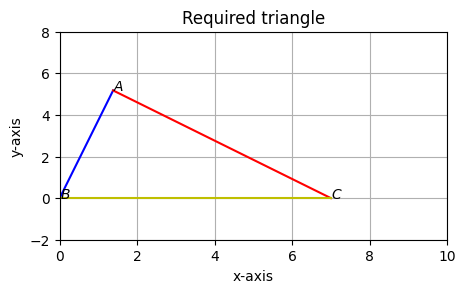
\includegraphics[width=\columnwidth]{chapters/const/examples/figs/2.png}
    \caption{}
    \label{fig:fig:1}
\end{figure}

\textbf{Solution :}
\begin{table}[H]
    \centering
      \begin{tabular}{|c|c|c|}
    \hline
    \textbf{Input parameters}&\textbf{Description}&\textbf{Value}\\
    \hline
    $\Vec{B}$&Vertex(at origin)&$\Vec{0}$ \\
    \hline
    $a$&Side of $\triangle ABC,BC$&$7$ \\
    \hline
    $b$&Side of $\triangle ABC,AB$&$b$ \\
    \hline
    $c$&Side of $\triangle ABC,AC$&$c$ \\
    \hline
    $\theta$&Angle of $\triangle ABC,\angle B$&$75\degree$ \\
   \hline
    \end{tabular}

    \caption{Table of input parameters}
    \label{tab:tab:1}
\end{table} 
\begin{table}[H]
    \centering
      \begin{tabular}{|c|c|c|}
    \hline
    \textbf{Output parameters}&\textbf{Description}&\textbf{Value}\\
    \hline
    $\Vec{C}$&Vertex&$ae_1$\\
    \hline
    $\Vec{A}$&Vertex&$c\begin{pmatrix}
        \cos{\theta}\\\sin{\theta}
    \end{pmatrix}$\\
    \hline
    $b+c$&$AB + AC$&13\\
    \hline
    \end{tabular}

  \caption{Table of output parameters}
    \label{tab:tab:2}
\end{table}


From appendix,
\begin{align}
    c&=\frac{k^2-a^2}{2\brak{k-a\cos{\theta}}}\\
    &=\frac{240}{52-7\sqrt{6}+7\sqrt{2}}
    \end{align}
Therefore,
\begin{align}
    \Vec{A}&=c\begin{pmatrix}
        \cos{\theta}\\\sin{\theta}
    \end{pmatrix}\\
    &=\frac{240}{52-7\sqrt{6}+7\sqrt{2}}\begin{pmatrix}
        \cos{75\degree}\\\sin{75\degree}
    \end{pmatrix}\\
    &=\begin{pmatrix}
        1.388\\5.18
    \end{pmatrix}\\
\end{align}
